\section{Résolution numérique}

Dans cette partie, nous allons expliquer comment le problème se résout
numériquement et aborder quelques considérations en rapport avec cette
résolution.

\subsection{Principe de la résolution}
La résolution peut être découpée en plusieurs partie, plus ou moins
indépendantes.

Une première considération numérique est la discrétisation spatiale du problème
: le disque sera représenté par un ensemble de position discrète selon l’axe
radial. Ces positions s’étendent de $x_\textrm{min} = \sqrt{r_\textrm{min}/r_s}$ à $x_\textrm{max} =
\sqrt{r_\textrm{max}/r_s}$, et sont séparées par un $\mathrm{d} x$ constant, ce qui aura pour
effet une fois revenu dans le monde dimensionné d’avoir un $\mathrm{d} r$ parabolique,
avec donc plus de points vers le bord intérieur du disque et moins vers le bord
extérieur. Comme l'instabilité commence par se développer au niveau du bord intérieur, il est favorable d'y avoir un bon échantillonnage.

\subsubsection{Courbe en S}

L’idée ici est de trouver les zones de stationnarité du système, c’est-à-dire
celles pour lesquelles la température évolue peu. Cela revient à résoudre
l’équation $Q^+ = Q^-$. En pratique, cette courbe a une forme « en S », avec
une partie arrondie correspondant au cas optiquement épais et une partie droite
correspondant au cas optiquement mince. Il y a deux points critiques : un au
point extrême de la partie arrondie, appelé premier point critique, et un au
point de jonction des deux parties, appelé second point critique.

Il faut donc déterminer la courbe de stationnarité en chaque point du disque,
puis sortir les coordonnées des points critiques pour chacun d’entre eux ainsi
que déterminer une position initiale pour le système sur ces courbes. Le détail de 
cette résolution sont donnés dans la partie \ref{sec:courbe_s}.

\subsubsection{Domaines de la simulation}

Le disque à un moment $t$ peut être dans l'une des trois situations suivantes.

\paragraph{Régime stationnaire} ce régime correspond au disque dans une
situation telle que tout le flux de matière entrant traverse le disque pour
finir par tomber dans le trou noir. Il est caractérisé par une température et
une densité surfacique constantes au cours du temps. Le taux d'accrétion est
alors constant et égal au taux d'accrétion à son bord extérieur. Numériquement,
il se traduit par une évolution relative de $T$ et $S^\star$ très faible entre
deux pas de temps. Lorsque ce régime est atteint, on augmentera le flux de
matière entrant au bord externe et ce jusqu'à ce qu'il n'y ait plus de régime
stationnaire.

\paragraph{Régime en évolution stable} ce régime correspond au disque évoluant
sur un temps visqueux pour la densité surfacique et un temps thermique pour la
température. Dans ce régime, on pourra négliger le terme advectif du chauffage.
Ce régime se situe dans la partie inférieure de la courbe en S et est
caractérisé par un quasi-équilibre thermique. On aura donc $Q^+ = Q^-$. Dans un
diagramme $\Sigma-T$, ce régime correspond au suivi de la partie inférieure
droite de la courbe en S. 

\paragraph{Régime en évolution instable} ce régime est celui de l'instabilité.
Il est caractérisé par une évolution de la densité surfacique et de la
température sur un même temps thermique. Dans ce régime, au moins une partie du
disque se situe à une température ou une densité de surface plus élevée que les
valeurs critiques. L'équilibre thermique n'y est alors pas atteint. C'est là
que se situe le cœur du problème. Le disque évacue de l'énergie par rayonnement
et perd beaucoup de matière par chute dans le trou noir. Chaque point proche du
point critique va effectuer des cycles autour du point critique. Ces points
voient d'abord leur densité augmentée jusqu'à dépasser la densité critique. Au
dela, la température croît rapidement jusqu'à ce que l'advection ne soit plus
négligeable et limite la température tout en diminuant la densité localement.
Le point se dirige alors vers les densités faibles, au dessus du point critique
jusqu'à retraverser la courbe en S, où le refroidissement est plus important
que le chauffage. Le point retombe alors dans la partie inférieure de la courbe
en S.

\subsubsection{Les conditions initiales}

Les relations nous permettant d'apporter des conditions satisfaisantes au
système sont données par les formules de Frank, King et Raine avec $P =
P_\textrm{gaz}$ et $\kappa_\textrm{ff} \gg \kappa_\textrm{e}$
\cite{F_K_R-1985}. Ces conditions en $\Sigma$ et $T$ sont suffisamment petites
pour ne pas influencer le système lors de son évolution. $\dot{M}$ est pris
très petit devant  le taux $\dot{M_{0}}$ imposé au système : 

\begin{equation}
	\dot{M} = 1\ 10^{-1 }\dot{M_{0}}
\end{equation} 

\begin{equation}
	T = 1.4 \times 10^{4} \alpha^{- \frac{1}{5}} \left[ \frac{\dot{M}}{10^{16} \mathrm{g.s}^{-1}} \right]^{\frac{3}{10}} \left[ \frac{M}{M_\odot}\right]^{\frac{1}{4}} \left[ \frac{r}{10^{10}\mathrm{cm}}\right]^{- \frac{3}{4}} f^{\frac{3}{10}} \mathrm{K} 
\end{equation}

\begin{align}
	\Sigma = 5.2 \alpha^{- \frac{4}{5}} \left[ \frac{\dot{M}}{10^{16} \mathrm{g.s}^{-1}} \right]^{\frac{7}{10}} \left[ \frac{M}{M_\odot}\right]^{\frac{1}{4}} \left[ \frac{r}{10^{10} \mathrm{cm}}\right]^{- \frac{3}{4}} f^{\frac{7}{10}} \mbox{K}  \\ 
	\text{avec } f = \left[ 1 - \left( \frac{r}{3 r_{s}}\right)^{- \frac{1}{2}}\right]
\end{align}

 \begin{figure}[ht]
   \begin{minipage}[c]{.46\linewidth}
      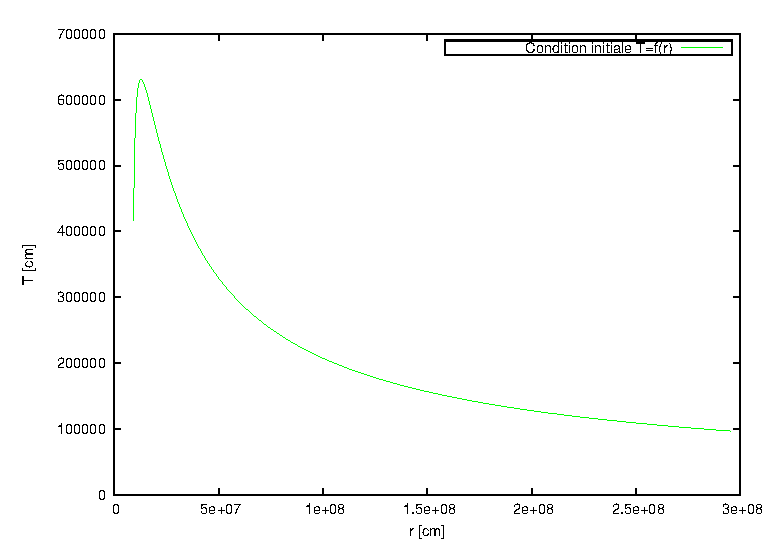
\includegraphics[scale=0.6]{ic_T.eps}
      \caption{Tracé de $T(r)$ à $t = 0$}\label{fig:CI_T}
   \end{minipage} \hfill
   \begin{minipage}[c]{.46\linewidth}
      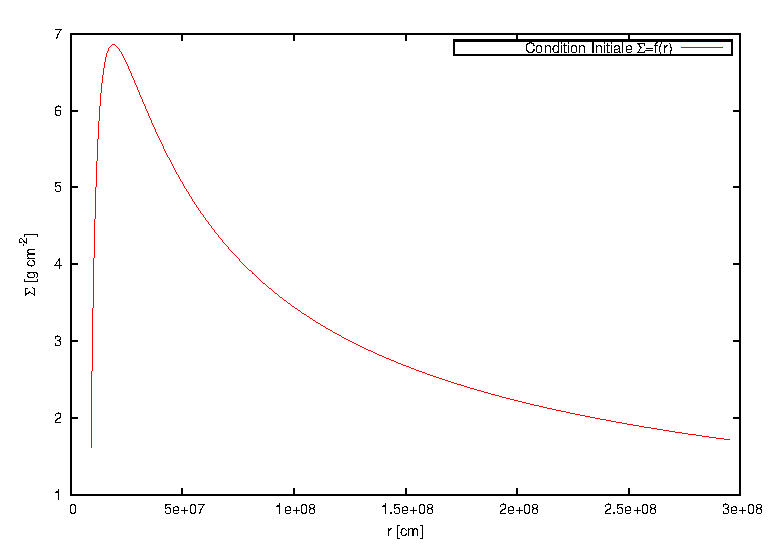
\includegraphics[scale=0.6]{ic_Sig.eps}
      \caption{Tracé de $\Sigma(r)$ à $t = 0$}\label{fig:CI_Sig}
   \end{minipage}
\end{figure} 

Nous pouvons voir sur les figures \ref{fig:CI_T} et \ref{fig:CI_Sig} les formes
de $T$ et $\Sigma$ en fonction de $r$ à l'instant initial.

Cela nous permet donc, à partir de l'utilisation du trinôme du second degré
explicité équation \eqref{eq:trinôme} de calculer la hauteur initiale du
disque. Dans le cas limite où s'expriment ces formules nous pouvons également
calculer le rapport $H/r$ à partir de la formule suivante : 

\begin{equation}
  \label{eq:H_r}
	\frac{H}{r} = 1.7 \times 10^{-2}\alpha^{- \frac{1}{10}} \left[ \frac{\dot{M}}{10^{16} \mbox{g} \mbox{s}^{-1}} \right]^{\frac{3}{20}} \left[ \frac{M}{M_\odot}\right]^{- \frac{3}{8}} \left[ \frac{r}{10^{10} \mathrm{cm}}\right]^{- \frac{1}{8}} f^{\frac{3}{5}}
\end{equation}
 
On peut alors comparer cette forme approximative avec la valeur simulée pour montrer que ces 
conditions initiales sont physiquement acceptables. Le tracé de cette courbe est effectué en figure \ref{fig:H_r}.

\begin{figure}
  \begin{center}
    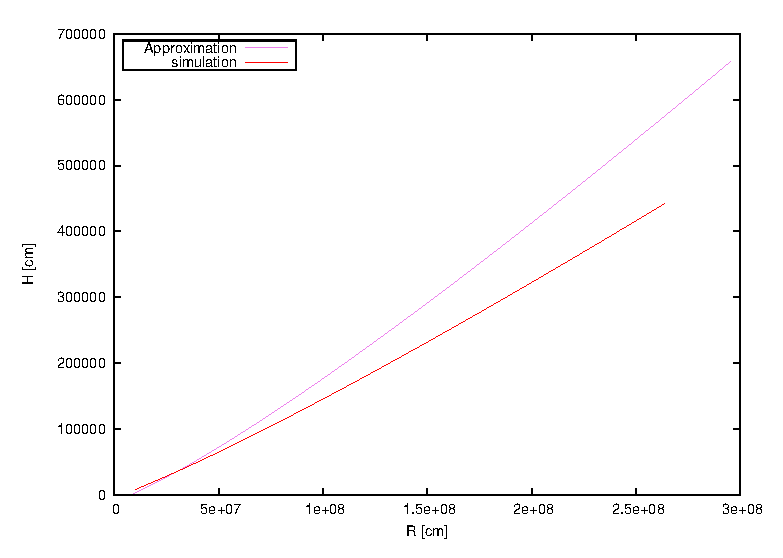
\includegraphics[]{ic_h.eps}
  \end{center}
  \caption{$H(r)$ à l'instant initial. La courbe rose est issue de la simulation, la courbe rouge est issue de l'équation \eqref{eq:H_r}}
  \label{fig:H_r}
\end{figure} 

Les deux formes étant toutes deux approximatives, on ne peut que comparer leurs
ordre de grandeurs qui sont compatibles. On supposera donc que les conditions
initiales sont physiquement raisonnables.

\subsubsection{Évolution du disque}

La simulation commence dans le régime en évolution stable et avec des
paramètres tels qu'un régime stationnaire existe. Le disque va alors rapidement
se stabiliser thermiquement jusqu'à atteindre la courbe en S avant de converger
sur un temps visqueux vers l'état stationnaire. Une fois l'état stationnaire
atteint, le flux de matière est augmenté. On recommence alors à suivre la
courbe en S jusqu'à atteindre un nouveau régime stationnaire.

Lorsque le flux de matière entrant est trop élevé, il n'existe plus de régime
stationnaire mais seulement un régime en évolution instable. Les points proches
des points critiques commencent alors à effectuer des cycles d'amplitude
croissante jusqu'à déclencher l'instabilité. Une fois l'instabilité terminée,
la densité et la température sont de nouveau assez faible pour retomber dans un
régime d'évolution stable.

\subsubsection{Intégration numérique de $S^\star$ et $T^\star$}

L'évolution du disque d'accrétion est dominé par les deux équations sur
$S^\star$ \eqref{eq:difS} et sur $T^\star$ \eqref{eq:difT}.

Les régimes stationnaires et en évolution stable seront traités avec un schéma
explicite pour la température et un schéma implicite pour la densité de
surface. On a alors un temps visqueux $\tau_\nu$ \FIXME{référence à une courbe,
une section?} (voir section \ref{sec::pas_de_temps}) très grand devant le temps
thermique $\tau_T$. On peut donc intégrer $S^\star$ et $T$ sur deux échelles de
temps différentes et effectuer une démarche de ``step and relax'', où on
intègre d'abord $S^\star$ sur un grand temps (visqueux) avant de laisser se
relaxer $T$ sur des petits temps (thermiques). Il faut à cet endroit faire
attention à ce que le temps de relaxation de $T$ soit toujours plus petit que
le temps visqueux. Cela revient à vérifier que le nombre d'itérations
nécessaires à la stabilisation de $T$ est plus petit que
$\nicefrac{\tau_\nu}{\tau_T}$. Si cette condition est violée, la simulation
numérique ne traduit plus de réalité physique. 

Une méthode implicite pour $S^\star$ est alors préconisée. En effet, celle-ci
assure de converger vers la solution et est stable quelque soit le pas de temps
(dans la limite des approximations données précédemment). Les détails de la
méthode sont donnés dans la partie \ref{ssec:integration_S_imp}. Pour intégrer
la température, il n'est pas possible d'écrire un schéma implicite. Il faudra
donc utiliser un schéma explicite. En revanche, il sera possible de procéder à
des simplifications pour donner une convergence plus rapide de $T$. Les détails
de ces approximations sont donnés dans la partie \ref{ssec:integration_T}.

L'autre régime est instable. Les évolutions de $S^\star$ et de $T$ se font sur
des temps similaires. Dans ce régime, il n'est plus légitime de traiter
séparement ces deux variables et il faut donc résoudre conjointement l'une et
l'autre. Le schéma implicite n'y est pas utilisé, car il n'assure que la
convergence vers une solution physique, mais pas via des états successifs
physiquement acceptables. Comme la valeur de $S^\star$ influe sur celle de $T$,
cela impliquerait que l'intégration de $T$ n'est pas non plus exacte. Dans le
cas du comportement chaotique de l'instabilité, il est nécessaire de limiter au
maximum les erreurs numériques car celles-ci peuvent mener à un résultat final
différent du résultat physiquement attendu. Le choix d'un schéma explicite est
alors fait pour $T$ et $S^\star$, les deux évoluant alors sur le plus petit
temps charactéristique du système : le pas de temps thermique. Le schéma
explicite est donné dans la partie \ref{ssec:integration_S_exp} pour $S^\star$
et dans la partie \ref{ssec:integration_T} pour $T$.

\subsubsection{Détermination du pas de temps\label{sec::pas_de_temps}}

Nous allons expliciter dans cette section les choix que nous avons fait pour
déterminer les différents pas de thermique $\tau_T$ et visqueux $\tau_\nu$
nécessaires aux intégrations en schéma implicite et explicite.

Sur la première branche (intégration en schéma implicite), ils sont déterminés
au cours de la simulation avant chaque nouvelle intégration en $S^\star$, à
partir des formules suivantes : 

\begin{equation}
	\Delta \tau_\nu^{imp} = \frac{\tau_\nu}{k_{\nu}} = \frac{1}{k_{\nu}} \times \frac{r}{v}
\end{equation}

\begin{equation}
	\Delta \tau_{T}^{imp} = \frac{\tau_{T}}{k_{T}}= \frac{1}{k_{T}} \times \frac{C_{V} T}{Q^{+} - Q^{-}}
\end{equation} \\

où $k_{\nu}$ et $k_{T}$ sont des constantes que l'on à prise respectivement égales à 100 et 1000.

Il est nécessaire dans cette simulation de faire intervenir un pas de temps
adaptatif. En effet, l'approche du point critique que l'on peut voir en figure
\ref{Fig::bench} est délicate. Le pas de temps visqueux est donc multiplier à
chaque nouvelle intégration sur $S^\star$ par un facteur $\alpha$ dépendant de la
distance au point critique par rapport à la variable $S^\star$. L'évolution du facteur $\alpha$ en fonction de la densité de surface $\Sigma$ est représenté figure \ref{fig::alpha_fct_sig} 


\begin{equation}
	\Delta^{'} \tau_{\nu}^{imp} = \alpha \Delta \tau_{\nu}^{imp}
\end{equation} \\

où $\alpha = 1 - \left( 0.99 \times \e^{- \left| \frac{S_\textrm{crit} - S}{D_\textrm{crit}} \right|} \right)$, avec $D_\textrm{crit}$ défini arbitrairement : $D_\textrm{crit} = 200$.


\begin{figure}
  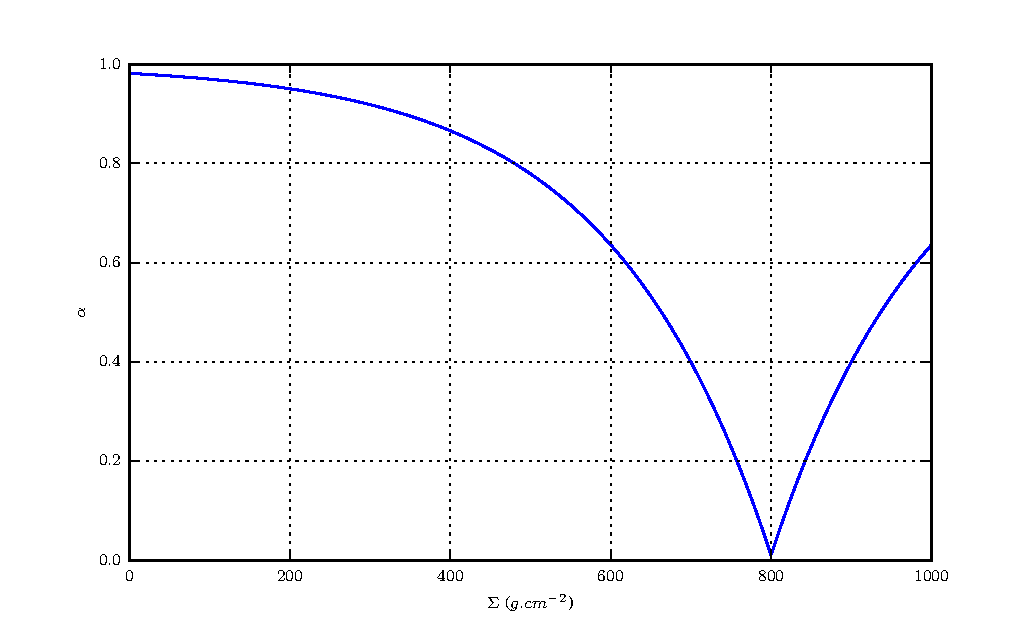
\includegraphics{figures/alpha_fonction_de_sigma.pdf}
  \caption{Evolution du facteur de ralentissement $\alpha$ en fonction de la densité de surface $\Sigma$ - Le point de rupture représente la valeur de $\Sigma$ au point critique}
  \label{fig::alpha_fct_sig}
\end{figure}

Le passage en shéma d'intégration explicite est soumis à deux conditions : $T
\ge T_\textrm{crit}$ ou $\Sigma \ge \Sigma_\textrm{crit}$. On bascule dès lors
qu'un des rayons à rempli ces conditions. $T$ et $\Sigma$ sont alors intégrés
sur le même pas de temps :

\begin{equation}
\Delta \tau_{T}^{exp} = 0.01 \times \Delta \tau_{T}^{imp}
\end{equation}

\subsubsection{Considérations sur les dérivées numériques spatiales}

Dans un certain nombre d’équations interviennent plusieurs dérivées spatiales,
du premier ou second ordre. Il existe plusieurs manières de les calculer
numériquement, ayant des conséquences variées. Nous nous intéresserons à
celles-ci dans cette partie afin d’expliquer les choix effectués.

\subsubsection{Conditions aux bords}

Toujours à propos des dérivées spatiales intervenant, l’existence de bords «
numériques » au problème implique d’imposer des conditions aux bords pour ces
dernières. Ces conditions dépendent des dérivées numériques utilisées, dans
cette partie seront présentées uniquement celles intervenant pour les dérivées
effectivement utilisées, les autres seront présentées en ANNEXE CL.
%TODO: Annexe CL

\subsubsection{Calcul des autres variables}


%\subsection{Courbe en S}
%\section{Détermination des courbes en S}

Nous avons voulu modéliser dans cette partie la condition d'équilibre thermique du plan équatorial du disque d'accrétion c'est-à-dire représenter l'état du système lorsque la quantité de chaleur produite ($Q^+$)est égale à la quantité de chaleur dissipée ($Q^-$), lorsque le terme de refroidissement est égal au terme de chauffage.
\begin{equation}
Q^+ = Q^-
\end{equation}
L'équation thermique devient donc, en négligeant le terme d'advection ($Q_{adv}$) qui représente la chaleur apportée ou emportée par la matière en mouvement.
\begin{equation}
Cv\frac{\partial T}{\partial t} = 0
\end{equation}
avec $Cv$ la capacité calorifique à volume constant par unité de masse du mélange de gaz et de radiation que l'on peut réécrire
\begin{equation}
\frac{\partial T}{\partial t} = 0
\end{equation}
Cette équation est stationnaire, elle ne dépend pas du temps mais elle dépend de la distante par rapport au centre du disque. Nous avons donc dû générer 256 courbes en S différentes pour chaque position du disque.

Nous avons voulu représenter sur un même graphique l'évolution de la température en fonction de densité de surface, c'est à dire représenter la fonction T($\Sigma$).
\\   

\subsection{Etablissement de la fonction}

Au premier abord, pour obtenir une seule courbe en S, le rayon r a été fixé. Ainsi la vitesse angulaire $\Omega$ a été préalablement définie. Par la suite nous avons répété la démarche suivante pour 256 différentes valeurs du rayon.
\\
En première partie, nous avons calculé la demi-hauteur H en utilisant la résolution d' une équation quadratique ne dépendant que de (T,$\Sigma,\Omega$) (Voir \ref{Equation}).
\\
Ensuite, la densité volumique $\rho$, la vitesse du son $c_s$ et la viscosité $\nu$. 
\\
De plus $\kappa_{ff}$, $\kappa_{e}$ et $\epsilon_{ff}$ pour pouvoir calculer le flux radiatif $F_z$ et déduire la différence des deux termes de chaleurs (en ne prenant pas en compte le terme d' advection) :
\\
\begin{equation} 
\label{eq:qplus-qmoins}
Q^+ - Q^- = 0. 
\end{equation}
\\
Nous avons aussi déterminé la profondeur optique effective $\tau_{eff}$. Selon sa valeur, nous pouvons nous placer dans un cas dit optiquement épais ($\tau_{eff} > 1$) ou bien dans le cas optiquement mince  ($\tau_{eff} < 1$).
Cependant nous ne l' avons pas utilisé comme critère pour le choix de l' expression du flux pour éviter de tomber sur des solutions stables artificielles qui seraient le fruit d' interpolations aux alentours de $\tau_{efff}$ = 1 où a lieu le basculement entre les deux approximations utilisées. 
\\
Nous avons donc calculé \ref{eq:qplus-qmoins} dans deux cas où on a imposé l' expression du flux radiatif. Ainsi, nous avons un algorithme où l' on peut fixer les valeurs de T et $\Omega$ pour obtenir une fonction ne dépendant que de $\Sigma$.

\subsection{Intervalle de température}
La résolution de la courbe en S nécessite de se placer dans un intervalle de température relativement restreint correspondant à la valeur de basculement de $\tau$ entre le cas optiquement épais et le cas optiquement mince.
Pour avoir un premier ordre de grandeur, nous nous sommes basés sur l'équation donnant la luminosité d'Eddington \ref{eq::} puis celle permettant de définir le taux d'accretion critique \ref{eq::} qui nous a donné la valeur de la température caractéristique $T_0$ de $1,40.10^6$ K. Nous avons ensuite, par paliers successifs, déterminé les intervalles de température permettant de représenter ce basculement d'état. Les deux valeurs que nous avons retenues sont : $T_{min}$ = 2,94.$10^5 K$ et $T_{max}$ 6,2.$10^6 K$ 
\\


\subsubsection{Méthode de la dichotomie}

Pour déterminer la densité de surface associée à une valeur de température précise, nous avons procédé par dichotomie.
Cette méthode consiste à trouver les coordonnées où s' annule une fonction continue en partant d' un intervalle de départ et en le divisant successivement pour cerner l' intervalle le plus petit possible où se trouve la solution.  
\\
Soit f(T,$\Sigma$) = $Q^+$ - $Q^-$ = 0,  une fonction continue et strictement monotone dans un intervalle [$\Sigma_{min}$ ; $\Sigma_{max}$] pour un T donné. Si f(T,$\Sigma_{min}$ ) et  f(T,$\Sigma_{max}$ ) sont de signes opposés, alors d' après le théorème de la bijection il existe une solution unique comprise dans cette intervalle. 
\\
Nous avons appliqué cette bissection en divisant à chaque fois l' intervalle en deux jusqu' à obtenir une solution avec une précision de $10^-6$ et en limitant le nombre d' itérations pour des raisons pratiques. Nous avons alors obtenu deux graphes, représentant T en fonction de $\Sigma$ pour un milieu optiquement épais (tracé courbé) et pour un milieu optiquement mince (relation linéaire).
\\

\begin{figure}[htb!]
\centering
\begin{tabular}{cc} 
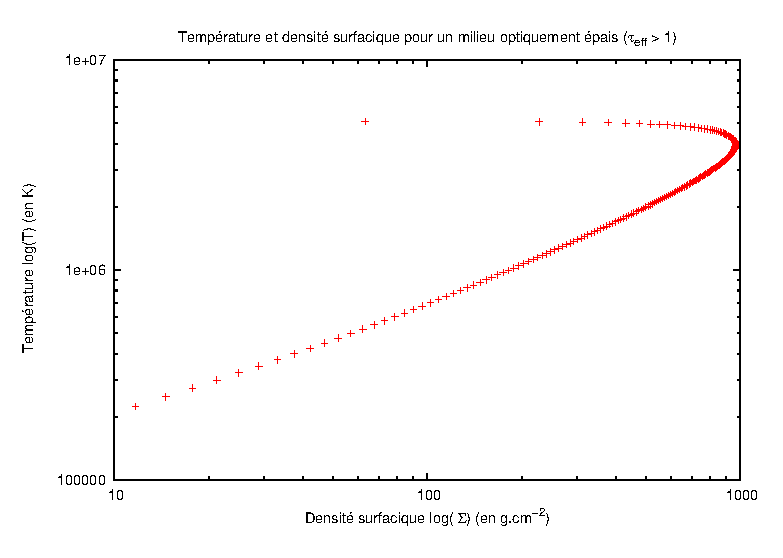
\includegraphics[height=0.3\textwidth]{S_curve_thick.eps} &
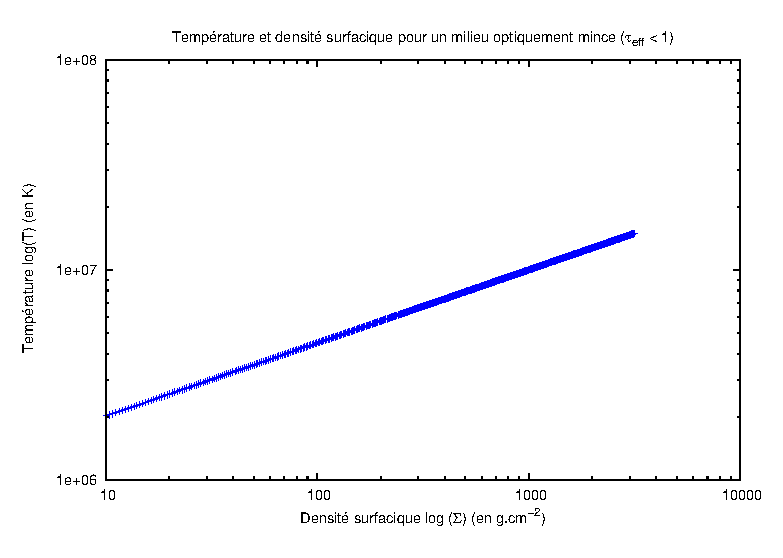
\includegraphics[height=0.3\textwidth]{S_curve_thin.eps} \\
\end{tabular}
  \caption{Cas optiquement épais (gauche) et optiquement mince (droite)}
\label{Fig::}
\end{figure}

La méthode de la dichotomie est une méthode simple et robuste pour trouver les "zéros" d'une fonction mais elle demande un grand nombre de d'itérations. En effet cette méthode converge linéairement.

Le nombre d'itérations par une méthode de dichotomie est donnée par la formule suivante : 
\begin{equation}
n = \frac{log(borne_{sup} - borne_{inf}) + log(\epsilon)}{log(2)} 
\end{equation}

Nous avons donc regardé s' il existait des méthodes qui convergeaient plus rapidement et de manière tout aussi robuste. 

\subsubsection{Méthode de Newton}
La méthode de Newton parfois appelée méthode de Newton-Raphson, décrite dans le \textit{De analysi per aequationes numero terminorum infinitas} en 1669. Cette méthode à l'avantage de converger beaucoup plus rapidement que pour la méthode de la dichotomie (convergence d'ordre 2)

\begin{equation}
x_{k+1} = x_k - \frac{f(x_k)}{f'(x_k)}
\end{equation}

En revanche, cette méthode présente plusieurs inconvénients, tout d'abord, la fonction doit être obligatoirement de classe $C^1$ et le calcul de la dérivée de manière analytique est complexe.


\subsubsection{Méthode de la sécante}

Un des gros inconvénient de la méthode de Newton est d'avoir à calculer la dérivée de la fonction. La méthode de la sécante permet de contourner cet obstacle et ne nécessite pas que la fonction soit de classe $C^1$

\begin{equation}
x_{n+1} = x_n - \frac{x_n - x_{n-1}}{f(x_n) - f(x_{n-1})}
\end{equation}

Cette méthode converge plus rapidement que la méthode de la dichotomie mais moins rapidement que la méthode de Newton (son ordre de convergence est compris entre 0 et 1 \footnote{Pour être plus précis l'ordre de convergence de cette méthode est égale à $\frac{1 + \sqrt{5}}{2}$} qui est le nombre d'or.). Elle permet également de s'affranchir également de la contrainte de l'intervalle de la fonction de la dichotomie. En revanche, cette méthode peut ne pas être robuste si la valeur initiale est trop éloignée de la solution ou s'il existe des racines multiples.

\begin{figure}[htb!]
	\centering
	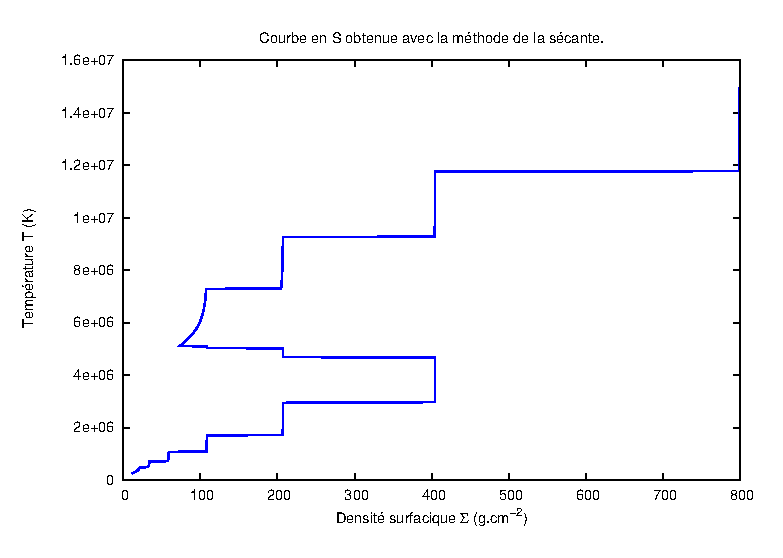
\includegraphics[height=0.7\textwidth]{S_curve_secant.eps}
	\caption{méthode de la sécante}
	\label{Fig::bench}
\end{figure}
%\FloatBarrier


\subsubsection{Méthode de Brent}
La méthode de Brent est une méthode de recherche de "zéros" d'une fonction combinant les méthodes de la dichotomie, de la sécante et l'interpolation quadratique inverse pour en utiliser tous leurs avantages. La méthode de l'interpolation quadratique inverse est une méthode de convergence rapide (ordre 2). Nous pouvons utiliser cette méthode si le dénominateur ne s'annule pas, c'est à dire :
\begin{equation}
f(b) \ne f(a) \text{ et } f(b) \ne f(c) 
\end{equation}
\begin{equation}
x = \frac{(y-f(a)(y-f(b))c}{(f(c)-f(a))(f(c)-f(b))} + \frac{(y-f(b)(y-f(c))a}{(f(a)-f(b))(f(a)-f(c))} +  \frac{(y-f(c)(y-f(a))b}{(f(b)-f(c))(f(b)-f(a))}
\end{equation}
Si cette condition n'est pas réalisée, nous utilisons la méthode de la sécante vue précédemment. Si la méthode de la sécante n'est pas efficace \footnote{C'est à dire.....}, nous utilisons la méthode de la dichotomie.
\\


\subsection{Comparaison des différentes méthodes}

\begin{figure}[htb!]
	\centering
	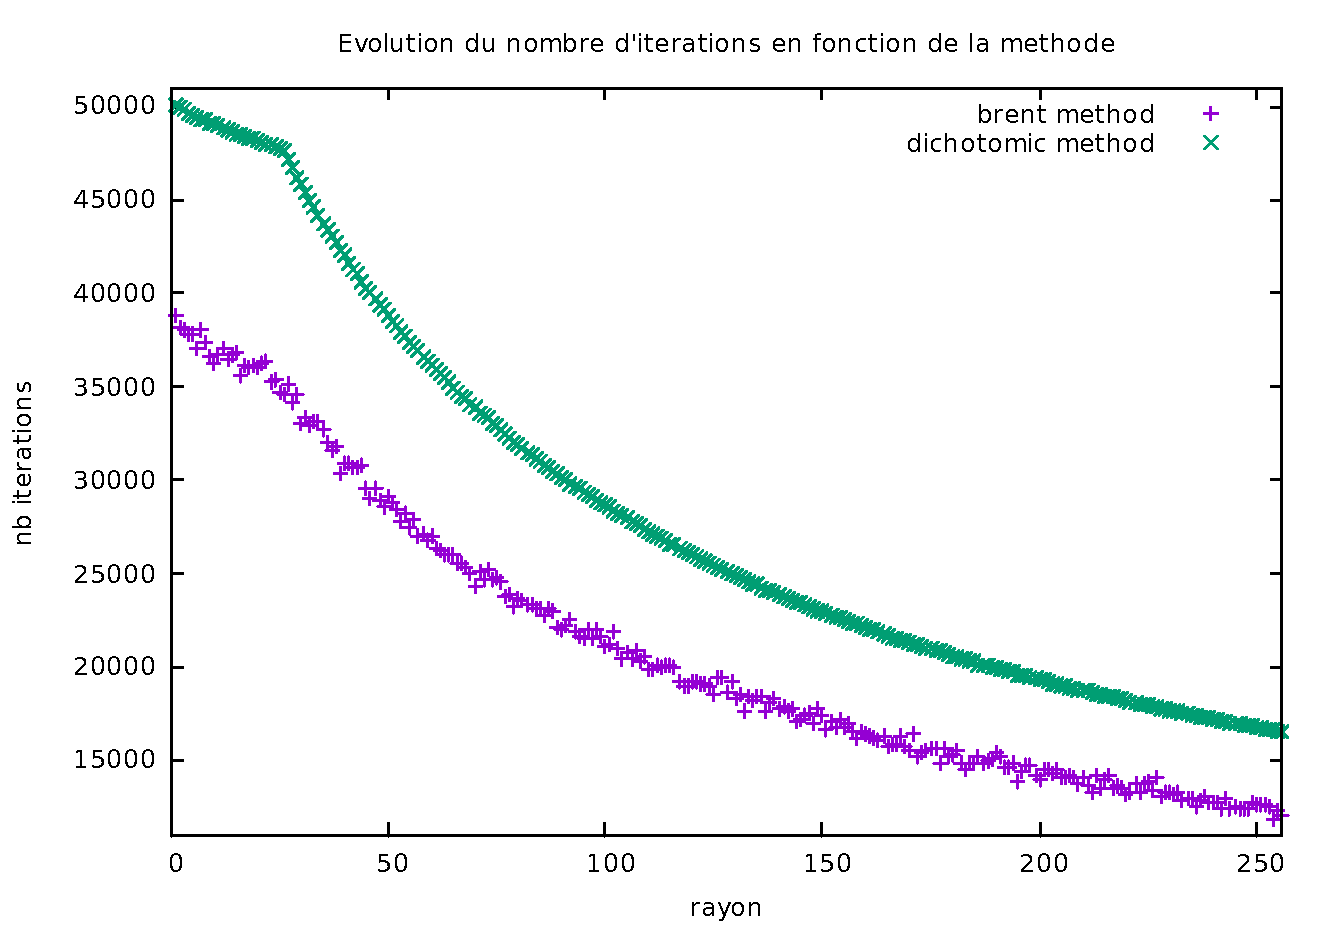
\includegraphics[height=0.5\textwidth]{brent_method3.pdf}
	\caption{Comparaison du nombre d'itérations nécessaire pour converger pour la méthode de la dichotomie et celle de Brent.}
	\label{Fig::bench}
\end{figure}


\subsection{Détermination des points critiques}
Afin de déterminer la propagation de l' instabilité thermique, il faut trouver le point critique où le système devient instable. Au niveau de la courbe en S, ceci a lieu sur la branche inférieure au niveau de la courbure : au-delà de ce point la densité surfacique diminue tandis que la température continue à s' élever. Sur la figure \ref{Fig::stable} la zone d'instabilité est représentée en bleue, les zones de stabilité sont en rouge.

\begin{figure}[htb!]
	\centering
	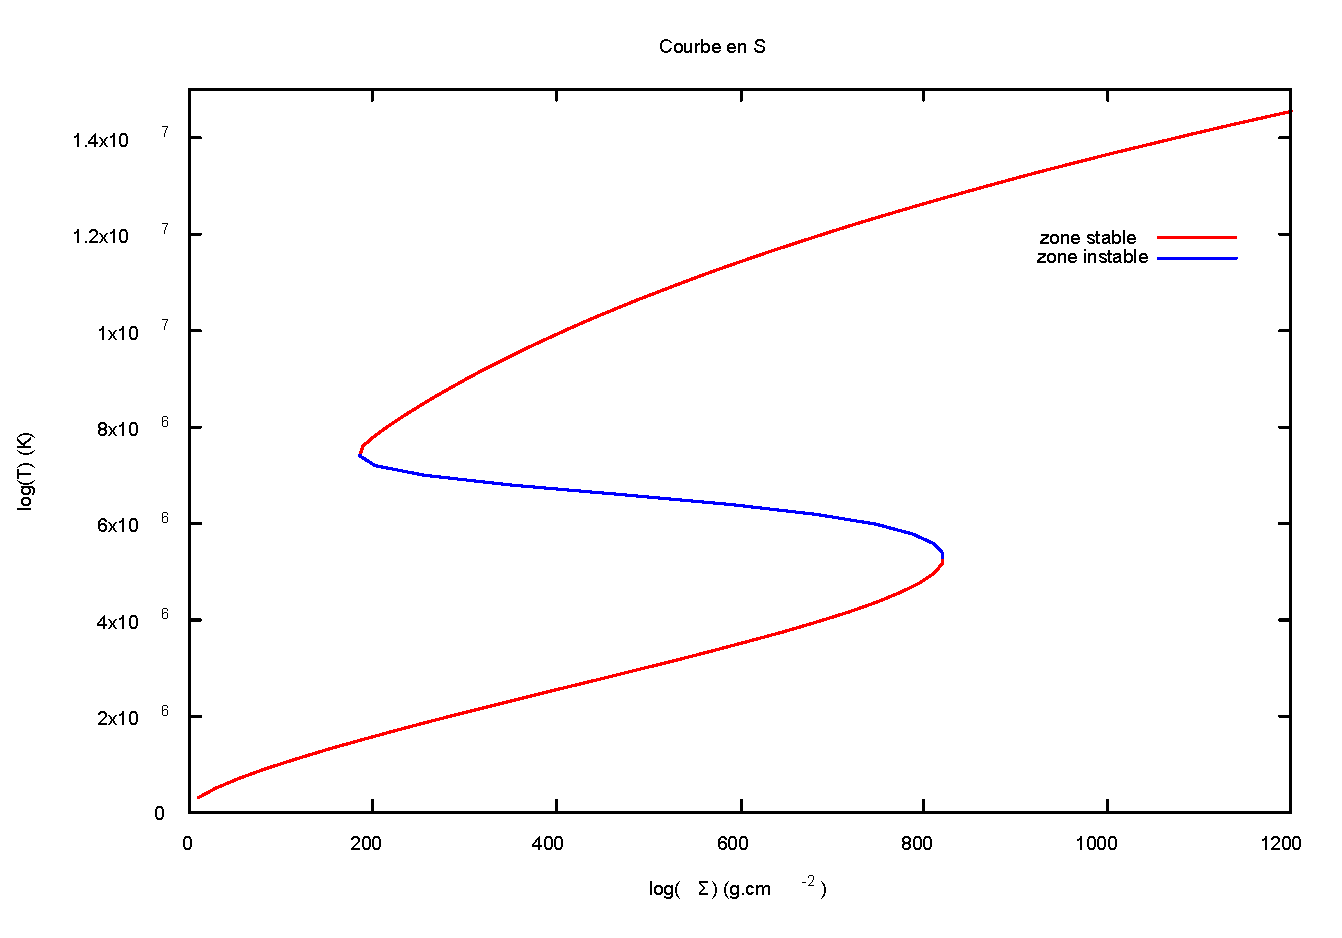
\includegraphics[height=0.7\textwidth]{stable.pdf}
	\caption{Zones stables et instables de la courbe en S}
	\label{Fig::stable}
\end{figure}
%\FloatBarrier

Nous pouvons voir sur ce schéma que la première zone de la courbe en S (la partie la plus basse) correspond à une position stable. Si l'on observe une petite élévation de température (si l'on se place légèrement au-dessus de la courbe), nous arrivons sur une zone ou le terme de refroidissement est supérieur au terme de chauffage, cette partie du disque va donc se refroidir pour retrouver sa position d'équilibre. De même, si l'on observe une petite diminution de température (si l'on se place légèrement en-dessus de la courbe) le terme de chauffage devient supérieur au terme de refroidissement, cette partie du disque va donc se réchauffer jusqu'à retrouver sa position d'équilibre. Il se passe exactement le même phénomène sur la partie haute de la courbe en S (zone III).

En revanche sur la partie centrale de la courbe (zone II), les petites perturbations se retrouvent amplifiées, nous sommes donc sur une section instable.


Pour trouver les coordonnées de ce point critique, nous avons comparé les valeurs de $\Sigma$ (calculé pour un milieu optiquement épais) pour chaque point en augmentant T. Lorsque la variation de la courbe change, c' est-à-dire quand $\Sigma$ cesse d' augmenter et commence à diminuer, nous avons repéré les coordonnées du dernier point pour lequel la densité surfacique croît.  
\\
Dans le code, nous avons nommé "deuxième point critique", le point où a lieu le basculement d'épaisseur optique. Sur les graphes, ce point se situe à l' intersection des deux branches et signale le changement de régime où on a utilisé une approximation de diffusion à une autre approximation où l'on doit prendre en compte les pertes par rayonnement de freinage (le refroidissement par bremsstrahlung).
\\
Pour le repérer, nous avons eu la même approche que pour pour le point d' instabilité trouvé préalablement. Cette fois-ci, nous avons comparé le $\Sigma$ déterminé pour un milieu optiquement épais à celui optiquement mince. Quand le premier devient plus petit que le second, celà signifie que la densité surfacique arrête de décroître et qu' elle commence à augmenter linéairement en fonction de la température. 
\\
%%%%%%%%[courbe en S avec les points légendés + ?evolution en fonction de r ?]

\subsection{Construction de la courbe}

En combinant les points trouvés dans le cas optiquement épais jusqu'au deuxième point critique et les points trouvés dans le cas optiquement mince, nous avons pu assembler les deux parties de la courbe en S.

\begin{figure}[htb!]
	\centering
	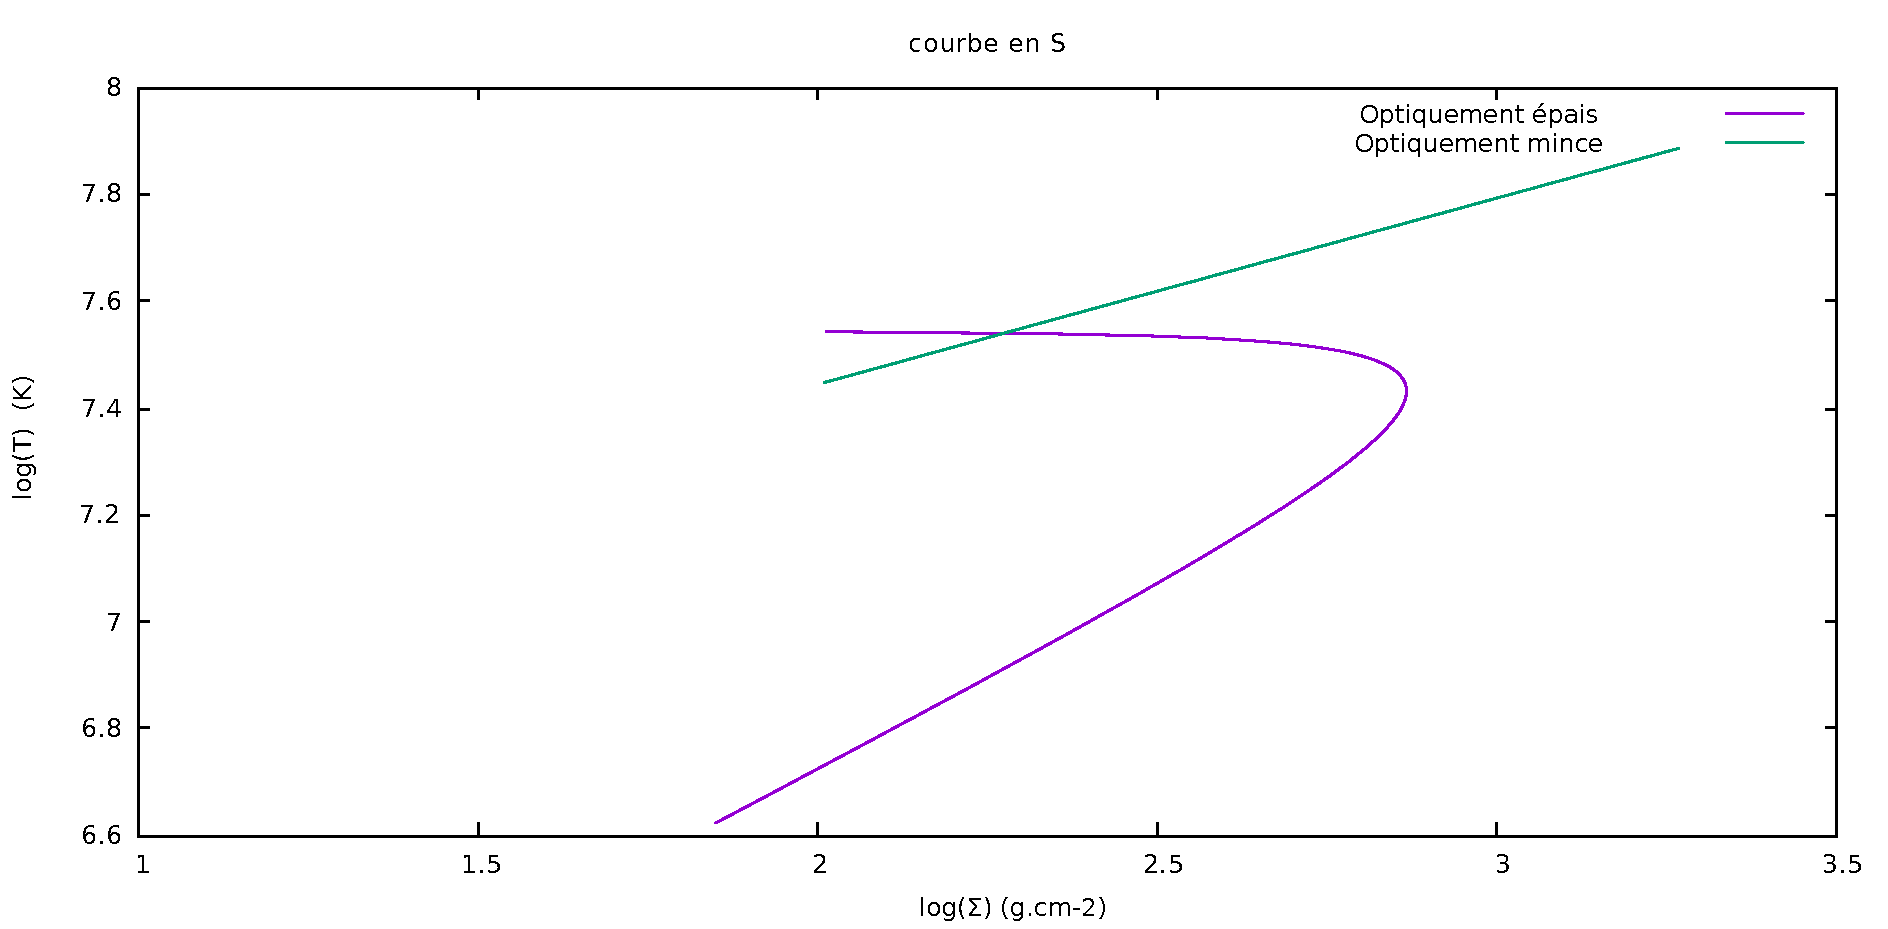
\includegraphics[height=0.5\textwidth]{deux_parties.pdf}
	\caption{Construction de la courbe en S}
	\label{Fig::bench}
\end{figure}


Nous avons donc pour chaque rayon une courbe en S représenté sur le graphe ci-dessous.
\begin{figure}[htb!]
	\centering
	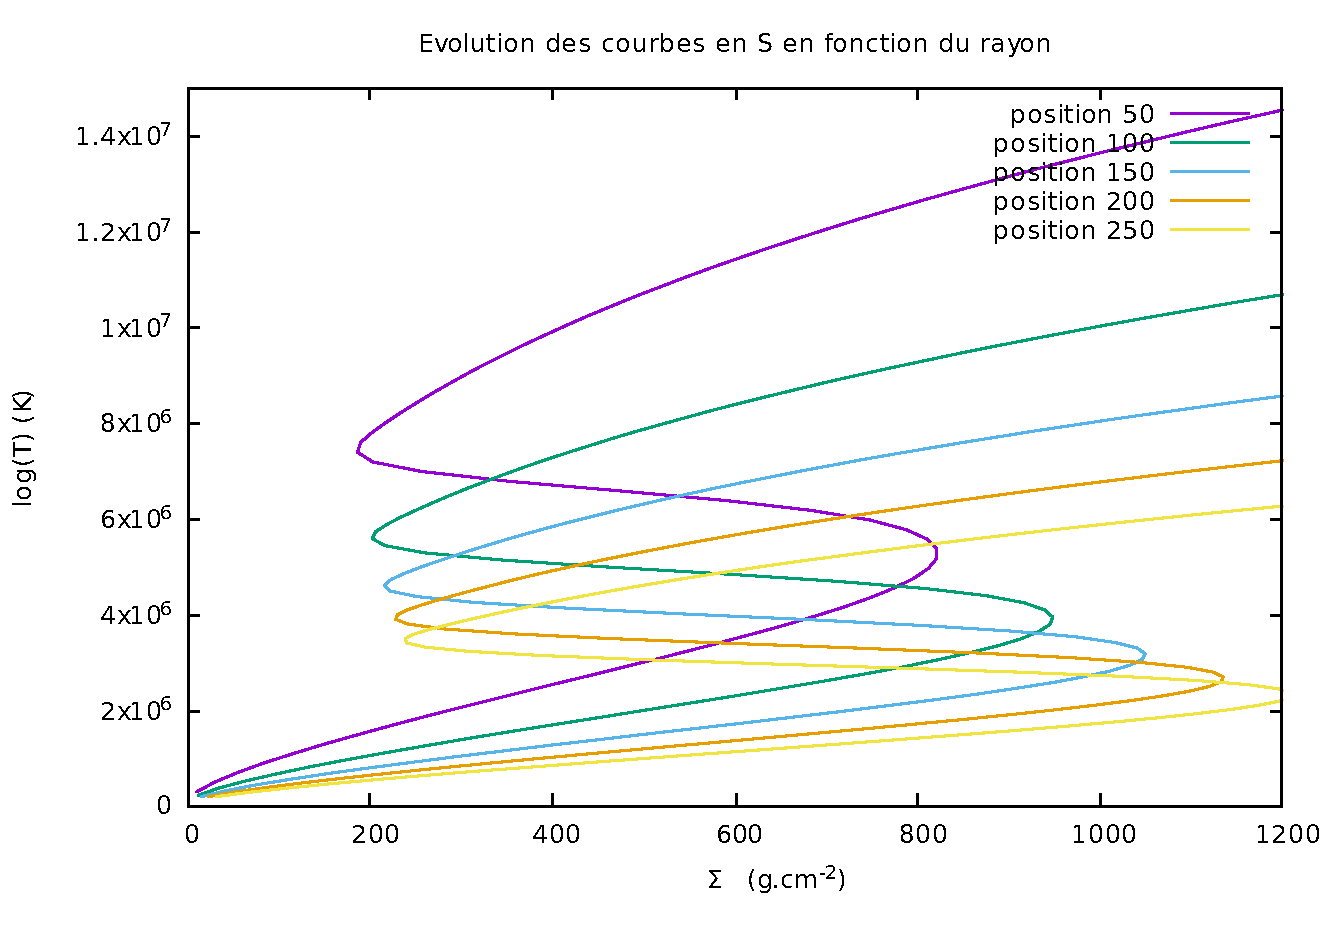
\includegraphics[height=0.7\textwidth]{evolutioncourbes.pdf}
	\caption{Evolution de la courbe en S en fonction de la distance au centre}
	\label{Fig::bench}
\end{figure}



\subsection{Evolution du $\tau_eff$}

D' après nos calculs nous trouvons un $\tau_eff$ aux alentours de 0,06 lors de la transition d'un milieu dit optiquement épais à un milieu optiquement mince. Cette valeur ne correspond pas à la valeur théorique où $\tau_eff$ = 1. 
Celà pose un problème au niveau de la partie d'intégration car notre branche linéaire est translatée par rapport à celle définie par la théorie. 
Cette différence de valeurs peut être expliquée par une erreur au niveau de l’adimensionnement ou bien dans les équations que nous avons utilisées ainsi que peut-être par une faute cachée dans nos paramètres ou nos constantes. 
\\
En fonction du rayon r, les coordonnées dans l' espace {T,$\Sigma$} des points ayant une valeur critique de $\tau_eff$ semblent évoluer de manière à ce que la température diminue et la densité surfacique augmente.
%%%manque d'inspiration  

\begin{figure}[htb!]
	\centering
	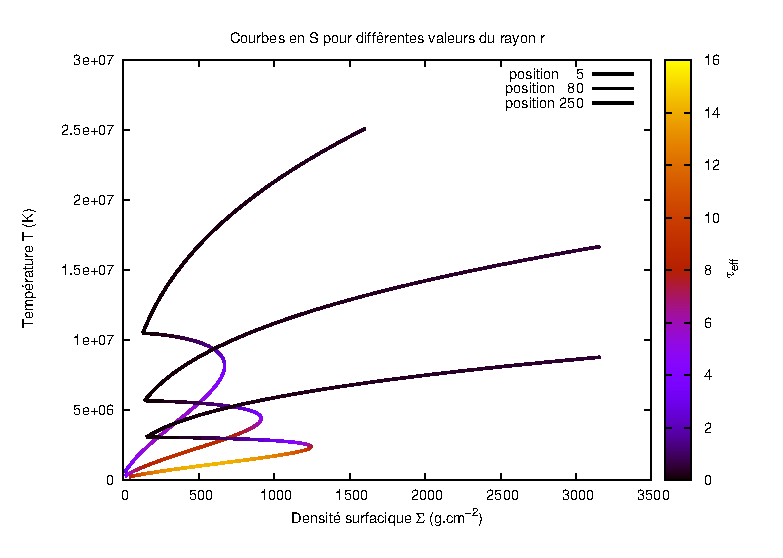
\includegraphics[height=0.7\textwidth]{S_curves_tau.eps}
	\caption{\textit{Evolution de la profondeur optique de la courbe en S pour diffèrents rayons.}  }
	\label{Fig::bench}
\end{figure}

\subsection{Pistes d'améliorations}

\begin{itemize}

\item Calcul direct $Q^+ = Q^-$
\\
Pour définir la température T en fonction de $\Sigma$, nous avons d' abord essayé de simplifier l' égalité $Q^+ = Q^-$ , qui traduit l' équilibre thermique local, en remplaçant tous les termes par T,$\Sigma$ et $\Omega$. Cela donne deux expressions (selon l'opacité du milieu) de fonctions implicites où ces variables sont couplées.
La résolution n' étant pas plus simple qu' avant le changement et afin d' éviter toute erreur induite lors du remplacement des différentes variables impliquées, nous avons préféré de calculer indépendamment chaque variable dans un ordre bien choisi. 
\\

\item Calcul des points critiques par dérivation de la fonction T($\Sigma$)
Comme nous n'avions pas à notre disposition une expression explicite d' allure T = f($\Sigma$), la dérivation des solutions issues d' une série d'équations ne semblait pas l'approche la plus efficace pour trouver le point critique d' instabilité. De plus, en dérivant nous aurions eu un problème au niveau du deuxième point critique qui est un point anguleux.
\end{itemize}

\subsection{Discussion}
Il n'est pas exclu qu'il existe plusieurs racines à l'équation $Q^+ = Q^-$, ce qui voudrait dire que la courbe en S n'est pas unique et plus particulièrement qu'il pourrait exister plusieurs branches dans le cas optiquement mince.

\subsection{Intégration numérique de S et T}\subsection{Intégration implicite de $S$}

\label{ssec:integration_S_imp}

L'intégration implicite revient à calculer $S^t$ en fonction de $S^{t+1}$, ce
qui donne un système linéaire qu'il est ensuite possible d'inverser. Il est
important de noter que cette méthode est plus coûteuse à chaque pas de temps
qu'une méthode explicite, car elle nécessite l'inversion d'une matrice. Il faut
donc vérifier que le gain de temps de calcul lié à une intégration sur un plus
grand pas de temps est plus important que le surcoût lié à l'inversion du
système.\FIXME{le faire …}. Dans la simulation, on vérifie systématiquement que
le temps de relaxation de $T$ est plus faible que le temps visqueux.

\paragraph{Linéarisation des équations}

On souhaite intégrer $S^\star$, la densité surfacique adimensionnée. L'équation
d'évolution est :

\begin{equation}
  \frac{\partial S^\star}{\partial t^\star} = \frac{1}{x^2}\frac{\partial^2}{\partial x^2}\left(\nu^\star S^\star\right)
\end{equation}

Pour alléger les notations, nous allons ommettre les étoiles dans les
développements prochains. L'équation s'écrit alors en passant aux variables
discrètes, au temps $t$ et à la case $1<n\leq n_\textrm{max}$

\begin{equation}
  \label{eq:S_discret_n}
  \frac{S^{t+1}_n - S^t_n}{\Delta t} = \frac{1}{x_n^2}\frac{\nu^t_{n+1}S^{t+1}_{n+1} - 2 \nu^t_nS^{t+1}_n + \nu^t_{n-1}S^{t+1}_{n-1}}{\Delta x^2}
\end{equation}

À l'intérieur du disque, la densité de matière est supposée nulle
($\nu^t_{0}S^{t+1}_{0} = 0$). Physiquement, il est en effet attendu qu'aucune
orbite keplerienne circulaire ne soit stable en dessous de l'ISCO
(\emph{\emph{I}nnermost \emph{S}table \emph{C}ircular \emph{O}rbit}), située en
$r = 3M$. En approximation, on suppose donc que la densité de matière y est
nulle.

\begin{equation}
  \label{eq:S_discret_1}
  \frac{S^{t+1}_1 - S^t_1}{\Delta t} = \frac{1}{x_1^2}\frac{\nu^t_{2}S^{t+1}_{2} - 2 \nu^t_1S^{t+1}_1}{\Delta x^2}
\end{equation}

Pour la case $n = n_\textrm{max} = N$, on a d'après \eqref{eq:nuS_n_is_null}:

\begin{equation}
  \frac{\nu^{t}_{N+1}S^{t+1}_{N+1} - \nu^{t}_NS^{t+1}_N}{\Delta x} = \dot{M}^\star_N
\end{equation}

Il faut noter que $\dot{M}^\star_N$ vaut initialement $1$. Pour simuler
l'arrivée de matière par l'extérieur du disque, cette quantité est incrémentée
au fur et à mesure de la simulation. Donc l'équation \eqref{eq:S_discret_n}
s'écrit en $N$:

\begin{equation}
  \label{eq:S_discret_N}
  \frac{S^{t+1}_N - S^t_N}{\Delta t} = \frac{1}{x_N^2}\frac{\Delta x - \nu^{t}_NS^{t+1}_N + \nu^{t}_{N-1}S^{t+1}_{N-1}}{\Delta x^2}
\end{equation}

\paragraph{Écriture matricielle}

On réécrit \eqref{eq:S_discret_n}, \eqref{eq:S_discret_1} et
\eqref{eq:S_discret_N} pour exprimer $S^t$ en fonction de $S^{t+1}$:

\begin{equation}
  \left\lbrace\begin{array}{r l c l c l }
    S^{t}_1 = &
               & &S_1^{t+1}\left(1 + 2\frac{\Delta t}{\Delta x^2}\frac{\nu_1^t}{x_1^2}\right)
               &+& S_{2}^{t+1}\left(-\frac{\Delta t}{\Delta x^2}\frac{\nu_{2}^t}{x_1^2}\right)\\
    S^{t}_n = &S_{n-1}^{t+1}\left(-\frac{\Delta t}{\Delta x^2}\frac{\nu_{n-1}^t}{x_n^2}\right)
               &+& S_n^{t+1}\left(1 + 2\frac{\Delta t}{\Delta x^2}\frac{\nu_n^t}{x_n^2}\right)
               &+& S_{n+1}^{t+1}\left(-\frac{\Delta t}{\Delta x^2}\frac{\nu_{n+1}^t}{x_n^2}\right)\\
    S^{t}_N + \frac{\Delta t}{\Delta x x_N^2} =
               &S^{t+1}_{N-1} \left(-\frac{\Delta t}{\Delta x^2}\frac{\nu_{N-1}^t}{x_N^2}\right)
               &+& S_N^{t+1} \left(1 + \frac{\Delta t}{\Delta x^2}\frac{\nu^t_N}{x_N^2}\right)
               & &
  \end{array}\right.
\end{equation}

Pour simplifier, on notera $A_k = 1 + 2 \frac{\Delta t}{\Delta x^2}\frac{\nu_k^t}{x_k^2}$ et $\Delta = \frac{\Delta t}{\Delta x^2}$
Ce système d'équation s'écrit aussi sous forme matricielle :
\begin{equation}
  \left(S^t\middle) + 
  \middle(\begin{matrix}
    0 \\
    \\
    \\
    \vdots \\
    \\
    \\
    \\
    0 \\
    \frac{\Delta t}{\Delta x}\frac{1}{x_N^2}
  \end{matrix}\middle)
  =
  \begin{pmatrix}
A_1                            & -\Delta\frac{\nu_{2}^t}{x_1^2} &  & & & & 0\\
-\Delta \frac{\nu_{1}^t}{x_2^2} & A_2                           & -\Delta\frac{\nu_{3}^t}{x_2^2} & & & &\\
    &        & \ddots                          &  & & & &\\
    &        & -\Delta \frac{\nu_{k-1}^t}{x_k^2} & A_k    & -\Delta \frac{\nu_{k+1}^t}{x_k^2} & &\\
    &        &                                 & & \ddots                          & & \\
    & & & & -\Delta \frac{\nu_{N-2}^t}{x_{N-1}^2} & A_{N-1} & -\Delta \frac{\nu_{N}^t}{x_{N-1}^2}\\
    0 & & & & & -\Delta \frac{\nu_{N-1}^t}{x_N^2} & 1 + \Delta \frac{\nu_N^t}{x_N^2}
  \end{pmatrix} \middle(S^{t+1}\right)
\end{equation}

Qui s'écrit aussi :

\begin{equation}
  AS^{t+1} = S^t + X 
\end{equation}

$A$ est une matrice tri-diagonale qu'il est facile de résoudre en utilisant Lapack (\href{http://www.netlib.org/lapack/explore-html/d4/d62/group__double_g_tsolve.html#ga2bf93f2ddefa5e671866eb2191dc19d4}{routine DGTSV}).
\FIXME{ajouter cela comme une référence}

\subsection{Intégration explicite de $S$}
\label{ssec:integration_S_exp}

Au contraire de l'intégration implicite, l'intégration explicite permet une
résolution directe d'une équation aux dérivées partielles. Il suffit de
connaître les variables à un temps $t$ pour en déduire la nouvelle valeur au
temps $t+1$ :

\begin{equation}
  S^{t+1} = S^t + \Delta t f(t)
\end{equation}
La solution au temps suivant est directement donnée.

\subsection{Intégration explicite de $T$}
\label{ssec:integration_T}

Il est possible d'améliorer le schéma d'intégration explicite pour la
température en donnant une meilleure estimation de $f(t)$.

\begin{equation}
  \frac{\partial T}{\partial t} = \frac{Q^+ - Q^- + Q_\textrm{adv}}{C_V} = f(T, S)
\end{equation}

On peut écrire un développement limité de $f(T) = f_0 + \frac{\partial
f}{\partial T}\Delta T + \frac{\partial f}{\partial S}\Delta S$ Comme on a un
temps thermique très petit devant le temps visqueux $\tau_\nu \gg \tau_T$
\FIXME{ est-ce vraiment vrai ?} , les variations de $f$ par rapport à $S$ sont
très faibles devant celles par rapport à $T$. On obtient alors $f(T) = f_0 +
f'_T \Delta T$. En linéarisant, on obtient finalement: \begin{equation} T^{t+1}
= T^t + \frac{f_0}{f'_T}\left[e^{f'_T\Delta t} - 1 \right] \end{equation} On
peut facilement obtenir numériquement une approximation de $f'_T$ en calculant
la quantité $\frac{f(T+\delta T) - f(T)}{\delta T}$, avec $\delta T = \lambda
T,\ \lambda \ll 1$.

\FIXME{ ajouter plot qui montre qu'on a bien df/dS << df/dT}
\FIXME{ajouter plot qui montre que la courbe est suffisamment lisse, c'est-à-dire que f'T peut bien être approximé numériquement}

\subsection{Considérations sur les dérivées numériques spatiales}

\FIXME{peut être bouger cette partie pour la cohérence ?}

Il existe un grand nombre de façon de dériver numériquement une variable $u$ en
fonction de l’espace discrétisé selon $r$ (pas spatial $\Delta{r}$). La plus
classique d’entre elles est celle des différences finies au premier ordre, qui
admet trois expressions standards~\eqref{eq:differences_finies}, qui exprime
$u_j = u(r,t)$ en fonctions des valeurs aux positions spatiales adjacentes
$u_{j+1} = u(r+\Delta{r},t)$ et $u_{j-1} = u(r-\Delta{r},t)$.

\begin{subequations}
    \label{eq:differences_finies}
    \begin{align}
        \label{eq:diff_droite}
        \frac{\partial u_j}{\partial r} &\approx \frac{u_{j+1} - u_j    }{  \Delta{r}}\\
        \label{eq:diff_gauche}
        \frac{\partial u_j}{\partial r} &\approx \frac{u_j     - u_{j-1}}{  \Delta{r}}\\
        \label{eq:diff_centre}
        \frac{\partial u_j}{\partial r} &\approx \frac{u_{j+1} - u_{j-1}}{2 \Delta{r}}
    \end{align}
\end{subequations}

Elles sont appelées respectivement \textit{différence à
droite}~\eqref{eq:diff_droite}, \textit{différence à
gauche}~\eqref{eq:diff_gauche} et \textit{différence
centrée}~\eqref{eq:diff_centre}. En pratique, la plus fidèle est celle des
différences centrées, mais elle n’est pas toujours utilisable.

En effet, considérons l’équation d’advection~\eqref{eq:advection_th} sous une
forme assez générale, où $v$ représente la vitesse d’advection (et donc son
signe le sens du gradient). 

\begin{equation}
    \label{eq:advection_th}
    \frac{\partial u}{\partial t} + v \frac{\partial u}{\partial r} = 0
\end{equation}

L’\cref{eq:advection_th} étant linéaire, on peut étudier la stabilité des
solutions numériques selon la méthode de Von Neumann. On considère $u(r,t)$ une
solution du problème et on ajoute une perturbation $\delta{u}$ à celle-ci. On
va alors regarder l’évolution de cette perturbation au cours du temps. La
linéarité nous permet de plus de considérer uniquement un terme de la
transformée de Fourier de $\delta{u}$, qu’on écrit alors $\delta{u} =
\tilde{u}(t) \e^{ikr}$. En réinjectant dans \eqref{eq:advection_th} et en
remplaçant $\frac{\partial u}{\partial r}$ par les expressions données
\cref{eq:differences_finies}, on obtient respectivement :

\begin{subequations}
    \begin{align}
        \frac{\partial \tilde{u}}{\partial t} \e^{ik\Delta{r}} &= - v \frac{\e^{ik(r+\Delta{r})} - \e^{ik r           }}{  \Delta{r}} \tilde{u}\\
        \frac{\partial \tilde{u}}{\partial t} \e^{ik\Delta{r}} &= - v \frac{\e^{ik r           } - \e^{ik(r-\Delta{r})}}{  \Delta{r}} \tilde{u}\\
        \frac{\partial \tilde{u}}{\partial t} \e^{ik\Delta{r}} &= - v \frac{\e^{ik(r+\Delta{r})} - \e^{ik(r-\Delta{r})}}{2 \Delta{r}} \tilde{u}
    \end{align}
\end{subequations}

En simplifiant ces équations par $\e^{ik\Delta{r}}$, cela devient :

\begin{subequations}
    \begin{align}
        \frac{\partial \tilde{u}}{\partial t} &= - v \frac{\e^{ik\Delta{r}} - 1                }{  \Delta{r}} \tilde{u}\\
        \frac{\partial \tilde{u}}{\partial t} &= - v \frac{1                - \e^{-ik\Delta{r}}}{  \Delta{r}} \tilde{u}\\
        \frac{\partial \tilde{u}}{\partial t} &= - v \frac{\e^{ik\Delta{r}} - \e^{-ik\Delta{r}}}{2 \Delta{r}} \tilde{u}
    \end{align}
\end{subequations}

On fait alors un développement limité en $ik\Delta{r}$ :

\begin{align}
    \e^{ ik\Delta{r}} &= 1 + ik\Delta{r} + \frac{i^2 k^2 \Delta{r}^2}{2}\\
    \e^{-ik\Delta{r}} &= 1 - ik\Delta{r} + \frac{i^2 k^2 \Delta{r}^2}{2}
\end{align}

Et on réinjecte :

\begin{subequations}
    \begin{align}
        \frac{\partial \tilde{u}}{\partial t} &= \left(- vik + v\frac{k^2}{2}\right) \tilde{u}\\
        \frac{\partial \tilde{u}}{\partial t} &= \left(- vik - v\frac{k^2}{2}\right) \tilde{u}\\
        \frac{\partial \tilde{u}}{\partial t} &= \left(- vik + 0             \right) \tilde{u}
    \end{align}
\end{subequations}

\begin{equation}
    \frac{\partial \tilde{u}}{\partial t} = - v \frac{2ik\Delta{r}}{2\Delta{r}} \tilde{u} = - i k v \tilde{u}
\end{equation}

\begin{equation}
    \tilde{u} = \tilde{u(0)} \exp(-i k v t)
\end{equation}

En fait, nous avons tout simplement :

\begin{equation}
    \frac{\exp(ik\Delta{r}) - \exp(-ik\Delta{r})}{2 \Delta{r}} = \frac{2 i \sin(k\Delta{r})}{2 \Delta{r}} = i k \sinc(k\Delta{r})
\end{equation}

Soit :
\begin{equation}
    \frac{\partial \tilde{u}}{\partial t} = - i k v \sinc(k\Delta{r}) \tilde{u}
\end{equation}

\begin{equation}
    \tilde{u} = \tilde{u(0)} \exp(-i k v \sinc(k \Delta{r}) t)
\end{equation}

\subsection{Conditions aux bords}

\subsection{Calcul des autres variables}

Pour chaque temps t donné, nous devons résoudre le système physique en chaque
point du disque. Cela correspond à résoudre un système de 16 équations et 16
inconnus \ref{sec::eq_adim}. Nous avons vu précédemment que toutes ces
quantités physiques nécessaires à  la simulation sont obtenues à  partir de
formules simples et immédiates, à  l'exception de la vitesse locale d'accrétion
$v$ ainsi que la demi-hauteur $H$ du disque.

\subsubsection{Résolution de la demi-hauteur $H$}
\label{ssec::resolution_H}

  $H$ fait en effet intervenir la résolution d'un trinôme du second degré dont nous avons détaillé le calcul ci dessous. \\

Partons de la pression P : 

\begin{equation}
	P = P_\textrm{gaz} + P_\textrm{rad}
\end{equation}


\begin{equation}
	c_{s}^{2} \rho = \frac{R \rho T}{\mu} + \frac{1}{3} a T^{4}
\end{equation}


\begin{equation}
	\Omega^{2} H^{2} \rho = \frac{R T}{\mu} \rho + \frac{1}{3} a T^{4}
\end{equation}


\begin{equation}
	\frac{1}{2} \Omega^{2} \Sigma H = \frac{R T}{\mu} \frac{\Sigma}{2 H} + \frac{1}{3} a T^{4}
\end{equation}

H est donc solution d'un trinôme du second degré $ a H^{2} + b H + c = 0$. \\
Compte tenu de l'adimensionnement considéré dans cette simulation, nous l'exprimons sous la forme suivante :  

\begin{eqnarray}
  a^{\prime} H^{* 2}+b^{\prime}H^{*}+c^{\prime}=0
  \end{eqnarray}

$\begin{cases}  
      a^{\prime} &= \Omega^{*2} \Omega_{0}^{2} S^{*} S_{0}\\
      b^{\prime} &= - \frac{2 a}{3 r_{s}} T^{*4} T_{0}^{4} x \\
      c^{\prime}&=-\frac{RT_{0}}{\mu r_{s}^{2}} T^{*} S^{*} S_{0}
     \end{cases}$ \\


\begin{equation}
	\Delta^{\prime} = b^{\prime 2} - 4a^{\prime}c^{\prime}
\end{equation} 

Il vient donc : 

\begin{equation}
	H^{*} = \frac{-b -sign(b) \sqrt{\Delta}}{2a}
\end{equation}


\subsubsection{Résolution de la vitesse locale d'accrétion $v$}
\begin{equation}
    v^\star = - \frac{1}{S^\star x} \frac{\partial}{\partial x} \left(\nu^\star S^\star\right)
\end{equation} 

Nous avons privilégié pour cette équation le calcul d'une moyenne des dérivées amonts et avales. La question de savoir lesquelles des dérivées (amonts ou avales) conduisent à  des solutions stables n'est pas nécessaire ici puisque en effet il ne s'agit pas d'une équation d'advection mais seulement d'une dérivée spatiale. Ci-dessous l'équation de la dérivée selon cette approximation : 

\begin{equation}
v^\star_{i} = - \frac{1}{S_{i}^\star x_{i}} \frac{( (\nu^{*}S^{*})_{i+1} - (\nu^{*}S^{*})_{i-1} )}{2 \Delta x_{i}}
\end{equation} 

Par contre ce choix de dérivée impose que nous mettions des conditions à  chaque bords du disque. La condition au bord intérieur est  $(\nu^{*}S^{*})_{0} = 0$, tandis que celle au bord extérieur est $v^\star_\textrm{max}   = - \dot{M^{*}}_\textrm{max} / (S^{*}x^{*})_\textrm{max}$.


\subsubsection{Ordre de résolution des équations}

Nous avons donc maintenant toutes les équations  nécessaires à  la résolution du système. L'ordre de résolution des équations est le suivant :  \\

 $\rightarrow$ Une foi le calcul de $H^{*}$ effectué, nous pouvons calculer les valeurs de la vitesse du son $cs^{*}$, de la viscosité $\nu^{*}$ ainsi que de la densité $\rho^{*}$ grâce aux formules décrites précédemment.   

 $\rightarrow$ Le calcul de $v$ nous permet quand à lui de trouver $\dot{M}$. Nous calculons également les valeurs de $\epsilon$,  $\kappa_\textrm{ff}$ et $\tau$, qui servent ensuite dans le calcul de $Fz$.
 
 $\rightarrow$ Enfin nous résolvons les équations des pressions $P_\textrm{gaz}$ et $P_\textrm{rad}$, de $\beta$,  de la capacité $Cv$ ainsi que des termes du transfert thermique $Q^{+}$, $Q^{-}$ et $Q_\textrm{adv}$.



%%% Local Variables:
%%% mode: latex
%%% TeX-master: "rapport"
%%% End:
